\subsection{\textit{k}mers and the \textit{k}mer Counting Problem} \label{background:kmers_and_kmer_counting}
A \textit{k}mer is a substring of \textit{k} consecutive nucleotides that occur in a DNA (or RNA) sequence.
Because of how single nucleotides can be represented in a computer's memory using only 2 bits \ref{background:nucleotide_binary_encoding}, and how when we sequence an individual's genome we can not know which strand our sequenced read comes from, a popular choice of value for \textit{k} is 31 - the default value used in KAGE \ref{background:kage}.
The value 31 is used in KAGE for two reasons: 1) having an odd value for \textit{k} ensures that no \textit{k}mer is equal to its reverse complement, and 2) having \textit{k} equals 31 means we need $31*2=62$ bits to represent the \textit{k}mer in a computer's memory, thus the \textit{k}mer will fit inside a single 64-bit integer.

A common problem in various bioinformatics applications is to count the number of times each valid \textit{k}mer in a set of nucleotide sequences occurs in those sequences.
This problem is commonly referred to as \textit{k}mer counting.

\definecolor{kmer1}{RGB}{40,40,215}
\definecolor{kmer2}{RGB}{0,150,0}
\definecolor{kmer3}{RGB}{225,30,30}
\definecolor{kmer4}{RGB}{20,150,150}

\begin{figure}[H]
\begin{center}
\scalebox{1}{
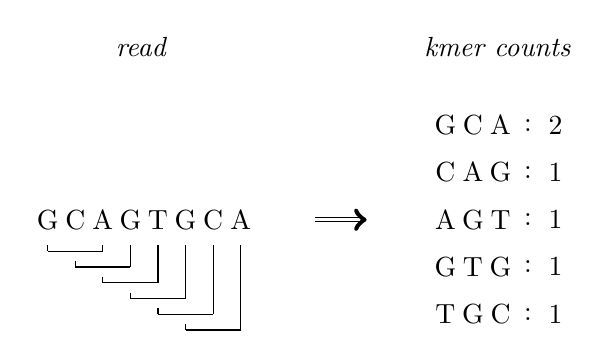
\begin{tikzpicture}
  % read
  %\node at(1.2,2.2)(){\fontfamily{phv}\selectfont\small read};
  \node at(1.2,2.2)(){\textit{read}};
  % sequence
  \node at(0,0){G};
  \node at(.35,0){C};
  \node at(.7,0){A};
  \node at(1.05,0){G};
  \node at(1.4,0){T};
  \node at(1.75,0){G};
  \node at(2.1,0){C};
  \node at(2.45,0){A};
  % kmer indicators
  % kmer 1
  \draw [](0,-.225-.1) -- (0,-.3-.1);
  \draw [](0,-.3-.1) -- (.7,-.3-.1);
  \draw [](.7,-.3-.1) -- (.7,-.225-.1);
  % kmer 2
  \draw [](.35,-.425-.1) -- (.35,-.5-.1);
  \draw [](.35,-.5-.1) -- (1.05,-.5-.1);
  \draw [](1.05,-.5-.1) -- (1.05,-.225-.1);
  % kmer 3
  \draw [](.7,-.625-.1) -- (.7,-.7-.1);
  \draw [](.7,-.7-.1) -- (1.4,-.7-.1);
  \draw [](1.4,-.7-.1) -- (1.4,-.225-.1);
  % kmer 4
  \draw [](1.05,-.825-.1) -- (1.05,-.9-.1);
  \draw [](1.05,-.9-.1) -- (1.75,-.9-.1);
  \draw [](1.75,-.9-.1) -- (1.75,-.225-.1);
  % kmer 5
  \draw [](1.4,-1.025-.1) -- (1.4,-1.1-.1);
  \draw [](1.4,-1.1-.1) -- (2.1,-1.1-.1);
  \draw [](2.1,-1.1-.1) -- (2.1,-.225-.1);
  % kmer 6
  \draw [](1.75,-1.225-.1) -- (1.75,-1.3-.1);
  \draw [](1.75,-1.3-.1) -- (2.45,-1.3-.1);
  \draw [](2.45,-1.3-.1) -- (2.45,-.225-.1);
  % arrow
  %\draw [thick,->](3.4,0) -- (4.05,0);
  \draw [double distance=1pt,->](3.4,0) -- (4.05,0);
  % k-mer counts
  %\node at(5.725,2.2)(){\fontfamily{phv}\selectfont\small kmer counts};
  \node at(5.725,2.2)(){\textit{kmer counts}};
  % kmer (count) representations
  % kmer 1
  \node at(5.05,1.2){G};
  \node at(5.4,1.2){C};
  \node at(5.75,1.2){A};
  \node at(6.1,1.2){:};
  \node at(6.45,1.2){2};
  % kmer 2
  \node at(5.05,.6){C};
  \node at(5.4,.6){A};
  \node at(5.75,.6){G};
  \node at(6.1,.6){:};
  \node at(6.45,.6){1};
  % kmer 3
  \node at(5.05,0){A};
  \node at(5.4,0){G};
  \node at(5.75,0){T};
  \node at(6.1,0){:};
  \node at(6.45,0){1};
  % kmer 4
  \node at(5.05,-.6){G};
  \node at(5.4,-.6){T};
  \node at(5.75,-.6){G};
  \node at(6.1,-.6){:};
  \node at(6.45,-.6){1};
  % kmer 5
  \node at(5.05,-1.2){T};
  \node at(5.4,-1.2){G};
  \node at(5.75,-1.2){C};
  \node at(6.1,-1.2){:};
  \node at(6.45,-1.2){1};
\end{tikzpicture}
}
\caption{
  \textit{Full} \textit{k}mer counting where we count the observed frequency of every valid 3-mer in our read set.
}
\label{background:kmers_and_kmer_counting:full_kmer_counting:figure}
\end{center}
\end{figure}

The genotyping software tool KAGE, detailed in section \ref{background:kage}, contains \textit{k}mer counting as one of its core steps in its genotyping pipeline.
However, the \textit{k}mer counting process in KAGE is slightly different from the process commonly refered to by the term \textit{k}mer counting.
Rather than counting the observed frequency of every valid \textit{k}mer in a set of input reads, KAGE only counts the observed frequencies of every \textit{k}mer in a predefined set.
Given how many valid \textit{k}mers one can observe in a set of hundreds of millions of reads, which is typical when sequencing and genotyping a human genome, not needing to store each of these with an associated count value makes this new \textit{k}mer counting variant significantly less memory and time consuming.

\begin{figure}[H]
\begin{center}
\scalebox{1}{
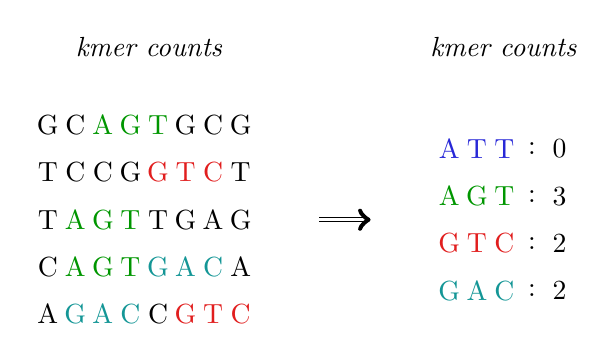
\begin{tikzpicture}
  % titles
  %\node at(-0.55+2.55,3)(){\fontfamily{phv}\selectfont\small kmer counts};
  \node at(-0.55+2.55,3)(){\textit{kmer counts}};
  % read 1
  \node at(-1.85+2.55,2){G};
  \node at(-1.5+2.55,2){C};
  \node at(-1.15+2.55,2){\textcolor{kmer2}{A}};
  \node at(-.8+2.55,2){\textcolor{kmer2}{G}};
  \node at(-.45+2.55,2){\textcolor{kmer2}{T}};
  \node at(-.1+2.55,2){G};
  \node at(.25+2.55,2){C};
  \node at(.6+2.55,2){G};
  % read 2 
  \node at(-1.85+2.55,1.4){T};
  \node at(-1.5+2.55,1.4){C};
  \node at(-1.15+2.55,1.4){C};
  \node at(-.8+2.55,1.4){G};
  \node at(-.45+2.55,1.4){\textcolor{kmer3}{G}};
  \node at(-.1+2.55,1.4){\textcolor{kmer3}{T}};
  \node at(.25+2.55,1.4){\textcolor{kmer3}{C}};
  \node at(.6+2.55,1.4){T};
  % read 3 
  \node at(-1.85+2.55,.8){T};
  \node at(-1.5+2.55,.8){\textcolor{kmer2}{A}};
  \node at(-1.15+2.55,.8){\textcolor{kmer2}{G}};
  \node at(-.8+2.55,.8){\textcolor{kmer2}{T}};
  \node at(-.45+2.55,.8){T};
  \node at(-.1+2.55,.8){G};
  \node at(.25+2.55,.8){A};
  \node at(.6+2.55,.8){G}; 
  % read 4 
  \node at(-1.85+2.55,.2){C};
  \node at(-1.5+2.55,.2){\textcolor{kmer2}{A}};
  \node at(-1.15+2.55,.2){\textcolor{kmer2}{G}};
  \node at(-.8+2.55,.2){\textcolor{kmer2}{T}};
  \node at(-.45+2.55,.2){\textcolor{kmer4}{G}};
  \node at(-.1+2.55,.2){\textcolor{kmer4}{A}};
  \node at(.25+2.55,.2){\textcolor{kmer4}{C}};
  \node at(.6+2.55,.2){A};
  % read 5 
  \node at(-1.85+2.55,-.4){A};
  \node at(-1.5+2.55,-.4){\textcolor{kmer4}{G}};
  \node at(-1.15+2.55,-.4){\textcolor{kmer4}{A}};
  \node at(-.8+2.55,-.4){\textcolor{kmer4}{C}};
  \node at(-.45+2.55,-.4){C};
  \node at(-.1+2.55,-.4){\textcolor{kmer3}{G}};
  \node at(.25+2.55,-.4){\textcolor{kmer3}{T}};
  \node at(.6+2.55,-.4){\textcolor{kmer3}{C}};
  % Arrow
  %\draw [thick,->](2.75,.8) -- (3.4,.8);
  \draw [double distance=1pt,->](4.15,.8) -- (4.8,.8);
  % k-mer counts
  %\node at(6.5,3)(){\fontfamily{phv}\selectfont\small kmer counts};
  \node at(6.5,3)(){\textit{kmer counts}};
  % k-mer 1
  \node at(5.8,1.7){\textcolor{kmer1}{A}};
  \node at(6.15,1.7){\textcolor{kmer1}{T}};
  \node at(6.5,1.7){\textcolor{kmer1}{T}};
  \node at(6.85,1.7){:};
  \node at(7.2,1.7){0};
  % k-mer 2 
  \node at(5.8,1.1){\textcolor{kmer2}{A}};
  \node at(6.15,1.1){\textcolor{kmer2}{G}};
  \node at(6.5,1.1){\textcolor{kmer2}{T}};
  \node at(6.85,1.1){:};
  \node at(7.2,1.1){3};
  % k-mer 3 
  \node at(5.8,.5){\textcolor{kmer3}{G}};
  \node at(6.15,.5){\textcolor{kmer3}{T}};
  \node at(6.5,.5){\textcolor{kmer3}{C}};
  \node at(6.85,.5){:};
  \node at(7.2,.5){2};
  % k-mer 4 
  \node at(5.8,-.1){\textcolor{kmer4}{G}};
  \node at(6.15,-.1){\textcolor{kmer4}{A}};
  \node at(6.5,-.1){\textcolor{kmer4}{C}};
  \node at(6.85,-.1){:};
  \node at(7.2,-.1){2};
\end{tikzpicture}
}
\caption{
  \textit{Partial} \textit{k}mer counting where we only count the observed frequencies of 3-mers present in a predefined set. In this example, our set of predefined 3-mers is \{ATT, AGT, GTC, GAC\}. During counting, 3-mers not present in this set are skipped.
}
\label{background:kmers_and_kmer_counting:partial_kmer_counting:figure}
\end{center}
\end{figure}

Henceforth in this thesis, we will in the favour of brevity refer to the former \textit{k}mer counting process where we count every valid \textit{k}mer's occurrence as \textit{full} \textit{k}mer counting, and to the latter process where we only count the occurrences of \textit{k}mers in a predefined set as \textit{partial} \textit{k}mer counting.

While several \textit{k}mer counting software tools have been developed in previous work, with at least one, Gerbil \cite{gerbil}, having support for GPU acceleration \cite{kmer_counting_tools}, these tools are designed to solve the \textit{full} \textit{k}mer counting problem.
